\section{Spherical geometry \& topology}
\label{sec:geometry}
The most fundamental object with which Driftworld Tectonics works is a mesh of a sphere in the 3D Euclidean space. For simplicity, we assume the sphere is a unit sphere centered on the origin unless stated otherwise. Because of the spherical nature of the project, several (arguably) uncommon mathematical concepts are described in this section -- such as vertex sampling, triangulation, transformations or bounding volume hiearchies. Although the text follows almost a textbook-like mathematical structure, a lot of the formulations and conclusions lack correct proof. Some reasoning is made to carry a~point, but meticulous readers are left to their own devices.
\subsection{Unity coordinate system}
\label{subsec:unitycoords}
Unity uses a left-handed coordinate system with the \textit{x} axis pointing to the right, \textit{y} axis pointing upwards and \textit{z} axis pointing forward (see Figure \ref{fig:unity-coordinate}). This is reflected in the scenes -- nevertheless, the mathematical expressions of vectors themselves are identical to a standard right-handed coordinate system, i. e. the following holds for the basis:
$$\mathbf{e}_x \times \mathbf{e}_y = \mathbf{e}_z$$
All implementations must be aware of the fact that the cross product expressions do not distinguish between right-handed and left-handed. It is simply a matter of axes display, where visually 'switching' axes \textit{y} and \textit{z} alternates between left-handedness and right-handedness. In the left-handed coordinate system, right-hand rule of cross product shows the inverse final direction of the cross product.
\begin{figure}[ht]
\centering
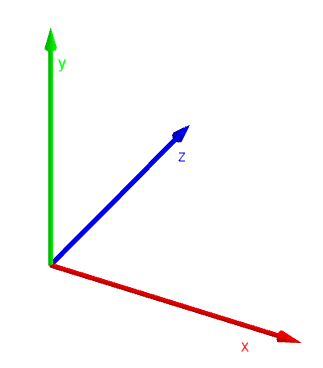
\includegraphics[height=7cm]{unity-axes.png}
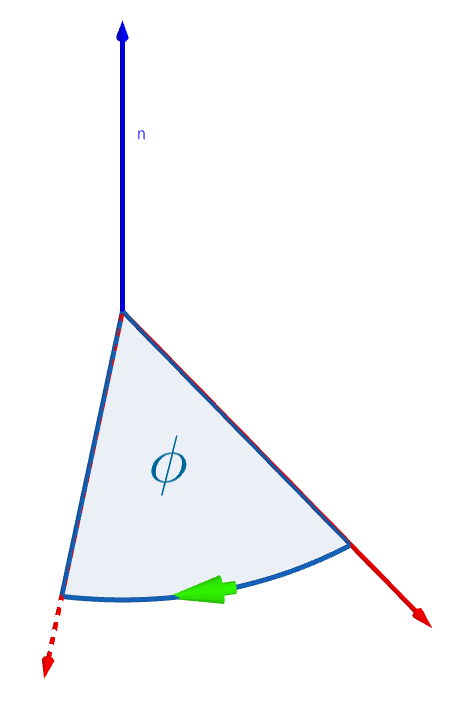
\includegraphics[height=7cm]{unity-rotation.png}
\caption{Unity coordinate system}
\label{fig:unity-coordinate}
\end{figure}

There are several ways to rotate points, vectors or whole transformations. For clarity, let us assume a 3-dimensional vector $\mathbf{u}$ that is to be rotated. We define a rotation unit vector $\mathbf{n}$ and an angle $\phi$ by which we rotate $\mathbf{u}$ so that $\mathbf{u}$ rotates by $\phi$ within a plane to which $\mathbf{n}$ is normal. We also assume that the rotation plane passes through the origin. Then from the perspective of a sundial (with $\mathbf{n}$ being the gnomon) $\mathbf{u}$ rotates \textit{clockwise} for positive $\phi$ (Figure \ref{fig:unity-coordinate}). This holds for all relative rotations.

\subsection{Sectional planes and great circles}
Sphere can have any number of sectional planes, i. e. planes that have some non-empty intersection with the sphere. Planes passing the center of the sphere will be called \textit{sectional central planes} (Figure \ref{fig:sectional-plane}). Any sectional central plane $\rho$ is characterized by some non-zero normal vector $\textbf{n}_\rho$ and for any point on the plane represented by their position vector $\mathbf{x}$ it holds that
$$\mathbf{n}_\rho\cdot\mathbf{x}=0$$
This is synonymous to the fact that any vector lying within a plane passing the origin is perpendicular to the normal vector of the plane. The dot product on the left side of the equality is also important because given a specific normal vector we can decide on which side is any vector $\mathbf{x}$ \textit{outside} the plane -- simply take the sign of the dot product, vector on the side of the normal vector will result in a positive dot product value with $\mathbf{n}_\rho$, negative otherwise.

An important object on the surface of a sphere is a great circle. It is any circle that shares its center and radius with the sphere (Figure \ref{fig:great-circle}). It is also the intersection of a plane passing the center of the sphere with its surface.
\begin{figure}[ht]
\centering
\begin{subfigure}{7cm}
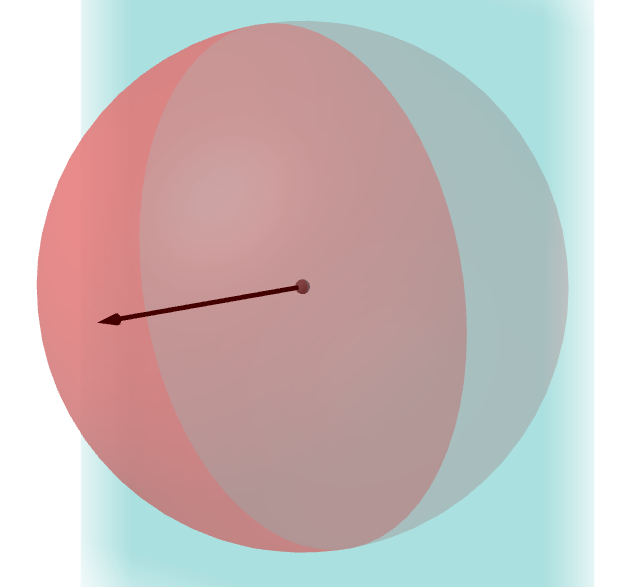
\includegraphics[height=6cm]{sectional-plane.png}
\caption{central plane}
\label{fig:sectional-plane}
\end{subfigure}
\begin{subfigure}{7cm}
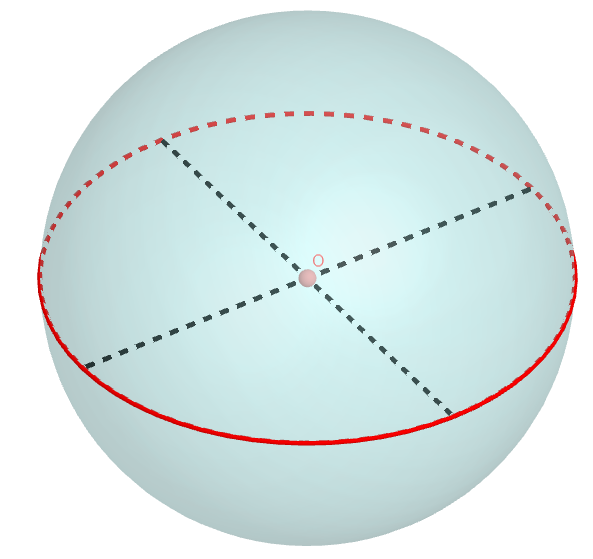
\includegraphics[height=6cm]{great-circle.png}
\caption{great circle}
\label{fig:great-circle}
\end{subfigure}
\caption{Sphere section by plane}
\label{fig:sectional-objects}
\end{figure}

\subsection{Spherical triangles}
Any three points on the surface of a sphere that do not lie on a single great circle form a~\textit{spherical triangle} (Figure \ref{fig:spherical-triangle}). This is the fundamental concept behind many of the computations in the project. However, strictly speaking, there are two triangles defined by such three points. The closure of the complement of any spherical triangle with respect to the sphere surface is also a spherical triangle, albeit one of the two is unintuitive as it is larger than half of the sphere surface area. To get around this, we construct somewhat narrower class of spherical triangles so that any three valid points define a triangle unambiguously.

\begin{figure}[ht]
\centering
\begin{subfigure}{8cm}
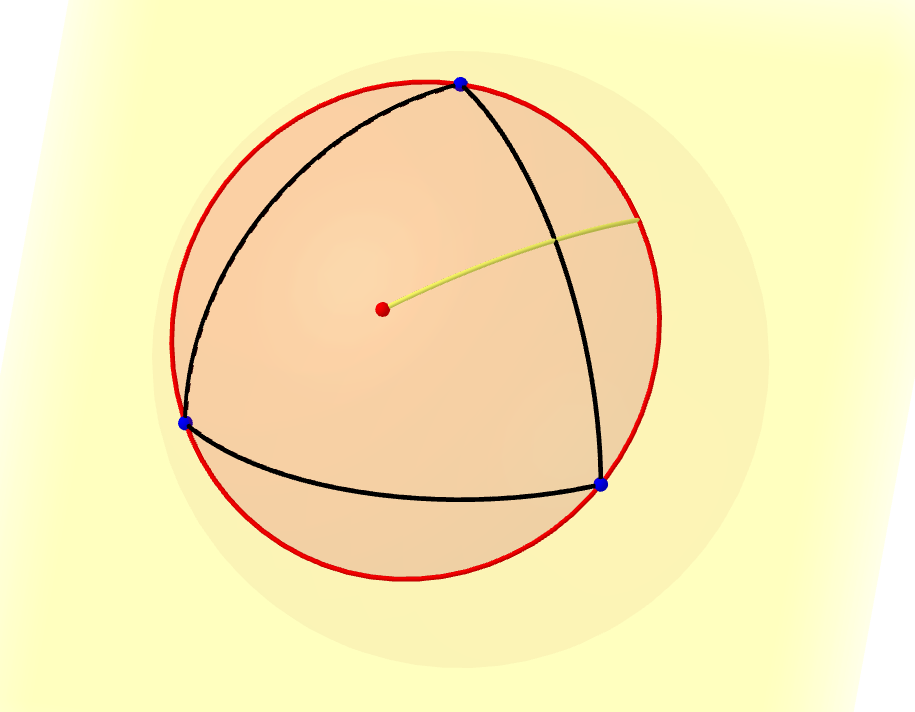
\includegraphics[height=6cm]{triangle-circumcircle.png}
\caption{with sectional plane and circumcircle}
\label{fig:triangle-circumcircle}
\end{subfigure}
\begin{subfigure}{8cm}
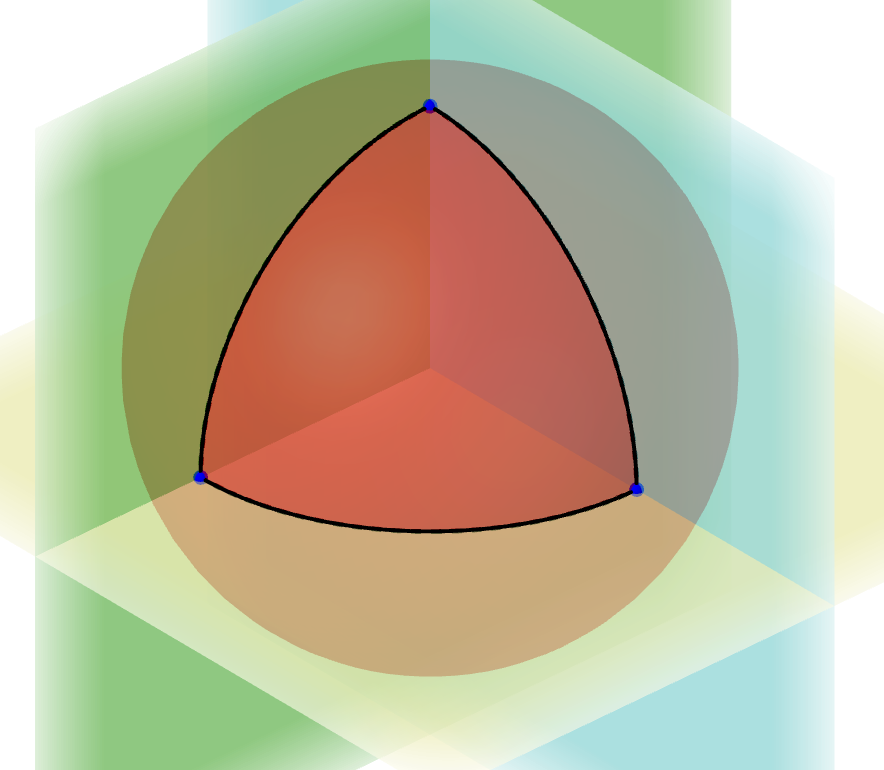
\includegraphics[height=6cm]{triangle.png}
\caption{planes intersections}
\label{fig:spherical-triangle-visual}
\end{subfigure}
\caption{Spherical triangle}
\label{fig:spherical-triangle}
\end{figure}

 We denote the surface of a unit sphere $\mathcal{S} =  \{\mathbf{x} \in \mathbb{R}^3: ||\mathbf{x}||=1\}$. Given a triplet of three linearly independent point vectors $(\mathbf{a},\mathbf{b},\mathbf{c})\in \mathcal{S}\times\mathcal{S}\times\mathcal{S}$ (called \textit{vertices})\footnote{Linear independence of unit vectors is equivalent to the condition that the vectors do not lie on a single great circle.}, we can construct a vector $\mathbf{n}_\lambda$ normal to some sectional plane $\lambda$ cutting off a spherical cap (Figure \ref{fig:sectional-plane}):
 $$\mathbf{n}_\lambda=(\mathbf{b} - \mathbf{a})\times(\mathbf{c} - \mathbf{a})$$
$$\forall\mathbf{x}\in\lambda: \mathbf{n}_\lambda\cdot\mathbf{x}+d_\lambda=0$$
We can calculate $d_\lambda$ by assigning e. g. $\mathbf{x}=\mathbf{a}$ and solving the plane equation with respect to $d_\lambda$, but that will not be neccessary. We impose a further requirement $\mathbf{n}_\lambda\cdot\mathbf{a}>0$. This is not always true, in which case it can be ensured by swapping any two vertices in the triplet and recalculating $\mathbf{n}_\lambda$. This means that all three vertices and their circumcenter are all 'on one side' of the sphere. In Unity coordinate system, this also means that for an outside observer, the vertices are oriented \textit{clockwise} on the sphere surface.

Spherical circumcircle $l$ is a set of points on a sphere that has constant spherical distance from a single point $\mathbf{c}_\mathcal{T}\in\mathcal{S}$ called \textit{circumcenter}. Equivalently, we can substitute dot product for distance:
$$\exists k\in\mathbb{R}:(\forall\mathbf{x}\in l:\mathbf{c}_\mathcal{T}\cdot\mathbf{x}=k)$$
Since $\mathbf{n}_\lambda\cdot\mathbf{a}=\mathbf{n}_\lambda\cdot\mathbf{b}=\mathbf{n}_\lambda\cdot\mathbf{c}>0$, we know that some scalar multiple of $\mathbf{n}_\lambda$ is the circumcenter for the vertices. In fact, there is only one possible circumcircle for all three vertices, which is the intersection $\mathcal{S}\cap\lambda$. We easily find the circumcenter and the circumradius $r_l$ as\footnote{We have to keep in mind that on a unit sphere, central angle and spherical distance are identical, barring formal dimension.}
$$\mathbf{c}_\mathcal{T}=\frac{\mathbf{n}_\lambda}{||\mathbf{n}_\lambda||}, r_l=\arccos(\mathbf{c}_\mathcal{T}\cdot\mathbf{a})$$

Previous reasoning allows us now to test if some point $\mathbf{x}\in\mathcal{S}$ is inside a spherical triangle $\mathcal{T}\subset\mathcal{S}$ with clockwise-oriented vertices $(\mathbf{a}, \mathbf{b}, \mathbf{c})$.
Geometrically speaking, a spherical triangle is a region bounded by three arcs of great circles \cite{palmer}. We calculate three normal vectors:
$$\mathbf{n}_{\rho}=\mathbf{a}\times\mathbf{b},$$
$$\mathbf{n}_{\sigma}=\mathbf{b}\times\mathbf{c},$$
$$\mathbf{n}_{\tau}=\mathbf{c}\times\mathbf{a}.$$
These vectors define planes $\rho, \sigma, \tau$ so that
$$\rho=\{\mathbf{x}\in\mathbb{R}^3:\mathbf{n}_{\rho}\cdot\mathbf{x}=0\}$$
$$\sigma=\{\mathbf{x}\in\mathbb{R}^3:\mathbf{n}_{\sigma}\cdot\mathbf{x}=0\}$$
$$\tau=\{\mathbf{x}\in\mathbb{R}^3:\mathbf{n}_{\tau}\cdot\mathbf{x}=0\}$$
intersections $\rho\cap\mathcal{S}, \sigma\cap\mathcal{S}, \tau\cap\mathcal{S}$ are then great circles that always pass two of the vertices. Because of this, each one is divided by them into two arcs. There is only one triplet of arcs connected by the vertices that forms a meaningful region boundary on $\mathcal{S}$ (Figure \ref{fig:spherical-triangle-visual}). There are two such regions but we already bypassed this problem by ensuring orientation. We test the point $\mathbf{x}$ against following condition:
$$\mathcal{T}=\{\mathbf{x}\in\mathcal{S}:\mathbf{n}_{\rho}\cdot\mathbf{x}\ge 0, \mathbf{n}_{\sigma}\cdot\mathbf{x}\ge 0, \mathbf{n}_{\tau}\cdot\mathbf{x}\ge 0\}$$
This simply tells us that $\mathbf{x}$ is inside the spherical triangle $\mathcal{T}$ when it is on the surface of the sphere and also on one specific side of all three planes $\rho, \sigma, \tau$. This definition does not encompass all possible spherical triangles on a sphere, but it allows us to properly test the properties of any triangles used in reasonable spherical meshes.
\subsection{Vertex sampling}
Because of memory restrictions, sphere surface data is represented as a set of sampled points. We can identify these points as position vectors $\mathbf{u}_i$ from the global origin to sample points, resulting in a~sequence $U=\left(\mathbf{u}_i\right)_{i=0}^{N-1}, \mathbf{u}_i \in \mathcal{S}$. Samples are therefore three-dimensional normalized vectors. Driftworld uses spherical Fibonacci sampling \cite{keinert}. To get the sequence $U$, another sequence $F=\left(\mathbf{f}_i\right)_{i=0}^{N-1}$ is first computed, using the following definition:
$$\mathbf{f}_i=(\phi_i, z_i), \phi_i \in \mathbb{R}, z_i \in \mathbb{R},$$
$$\phi_i = 2\pi\left[\frac{i}{\Phi}\right],$$
$$z_i = 1-\frac{2i+1}{N}.$$
$\left[x\right]$ denotes the fractional part of $x$, $\Phi$ is the golden ratio $\Phi=\frac{\sqrt{5}+1}{2}$. The values of $\mathbf{f}_i$ actually lie on a~spiral on the surface of a cylinder with the radius of 1 and the height of 2 \cite{keinert}. $U$ is finally obtained by mapping $\mathbf{f}_i$ values to $\mathcal{S}$:
$$\mathbf{u}_i = (\sin{(\arccos{(z_i)})}\cdot\cos{\phi_i}, z_i, \sin{(\arccos{(z_i)})}\cdot\sin{\phi_i})$$
Note that this mapping reflects Unity's axes orientation and the first and the last samples of $U$ do not fall exactly on the poles.
\subsection{Centroids, data values and barycentric interpolation}
Driftworld often makes computations for points inside sperical triangles - notably, it uses triangle centroids to evaluate triangle neighbours. Calculating these points is not a trivial procedure and although for a long time there have been methods to do so, it would be too resource-consuming when performed on a larger scale. To save computation time, we assume that all evaluated triangles are nearly planar, i. e. their \textit{triangle excess} is negligible (Legendre's Theorem\footnote{This theorem is also known as Saccheri-Legendre theorem.} \cite{todhunter}). We calculate the centroid of a triangle by simply normalizing the sum of its vertices (Figure \ref{fig:triangle-centroid}):
$$\mathbf{b}_\mathcal{T}=\frac{\mathbf{a} + \mathbf{b} + \mathbf{c}}{||\mathbf{a} + \mathbf{b} + \mathbf{c}||}$$
\begin{figure}[ht]
\centering
\begin{subfigure}{7cm}
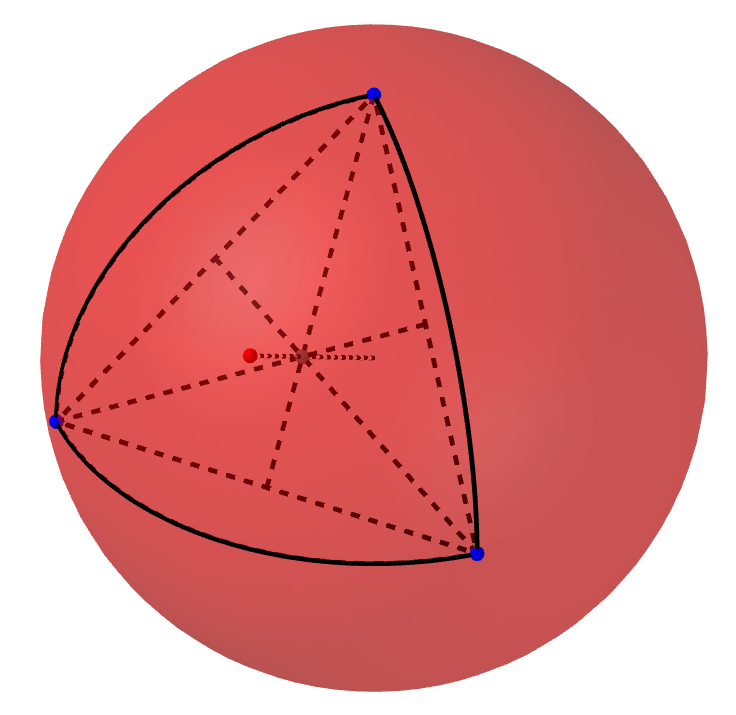
\includegraphics[height=6cm]{triangle-centroid.png}
\caption{sectional triangle centroid}
\label{fig:triangle-centroid}
\end{subfigure}
\hspace*{1cm}
\begin{subfigure}{7cm}
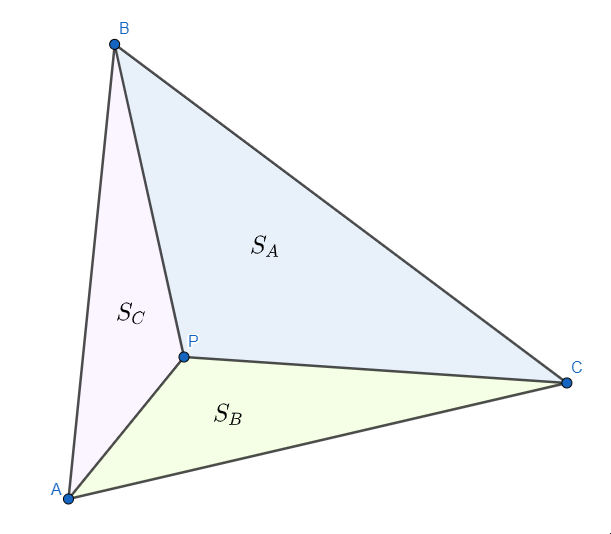
\includegraphics[height=6cm]{triangle-barycentric.png}
\caption{barycentric coordinates}
\label{fig:triangle-barycentric}
\end{subfigure}
\caption{Centroid geometry}
\label{fig:centroid-geometry}
\end{figure}

To store crust data, we must assign values to points on the sphere. These values may be of different types or have different meaning. Formally, we denote a sequence of arbitrary sets $C=\left(V_i\right)_{i=0}^{n-1}$, where $n$ is the number of different values assigned to a point and each $V_i$ is a specific of value. The system of all possible value combinations is then a cartesian product of these value sets:
$$V=\prod_{i=0}^{n-1}V_i$$
Stored data can then be defined as a map:
$$s: U\rightarrow V$$
$$s_i: U\rightarrow V_i$$
We store data only for sphere samples because of limited memory. Other values will be computed as needed using \textit{barycentric interpolation} \cite{scratchapixel}.\newpage

Now it comes to the following problem: how to compute values anywhere on $\mathcal{S}$? We are effectively looking for some domain extension, since $U\subset\mathcal{S}$:
$$s':\mathcal{S}\rightarrow V, \forall \mathbf{u}\in U:s'(\mathbf{u})=s(\mathbf{u})$$
$$s_i':\mathcal{S}\rightarrow V_i, \forall \mathbf{u}\in U:s_i'(\mathbf{u})=s_i(\mathbf{u})$$
Given some arbitrary point $\mathbf{x}\in\mathcal{S}$, we start with an assumption that $\mathbf{x}$ is found inside some spherical triangle $\mathcal{T}$ with negligible triangle excess and vertices $\{\mathbf{a}, \mathbf{b}, \mathbf{c}\} \subset U$ for which we already know the values of $s$. We would like $s'(\mathbf{x})$ to be computed 'fairly', i. e. the closer $\mathbf{x}$ is to some vertex, the more influence the vertex value should have on $s'(\mathbf{x})$. A good start might be in analogy with a political voting system based on area. If the population is homogeneous, any region vote is weighted by its area and transitionally, by its population.

Let $P$ be some point within a triangle $ABC$ (Figure \ref{fig:triangle-barycentric}). This point is represented by a point vector $\mathbf{p}\in\mathcal{S}$. As stated earlier, we assume all points lie nearly on the same plane. If we construct three triangles $PBC$, $APC$ and $APB$, the triangle $ABC$ will be divided into three regions, each corresponding to their oposite vertex of $ABC$. The closer $P$ is to any of the vertices, the larger the corresponding triangle area is. Total area sum of the three triangles is equal to the area of $ABC$. Therefore, we can use these triangle areas as weights for interpolating values at $P$ -- we only need to find the respective areas of $S_A, S_B, S_C$ and $S_{ABC}$. This can be done using cross product:
$$S_A=\frac{|(\mathbf{b}-\mathbf{p})\times(\mathbf{c}-\mathbf{p})|}{2}$$
$$S_B=\frac{|(\mathbf{c}-\mathbf{p})\times(\mathbf{a}-\mathbf{p})|}{2}$$
$$S_C=\frac{|(\mathbf{a}-\mathbf{p})\times(\mathbf{b}-\mathbf{p})|}{2}$$
$$S_{ABC}=\frac{|(\mathbf{b}-\mathbf{a})\times(\mathbf{c}-\mathbf{a})|}{2}$$
Since $S_A+S_B+S_C=S_{ABC}$, we can define normalized weights $u, v, w$ called \textit{barycentric coordinates}:
$$u=\frac{|(\mathbf{b}-\mathbf{p})\times(\mathbf{c}-\mathbf{p})|}{|(\mathbf{b}-\mathbf{a})\times(\mathbf{c}-\mathbf{a})|}$$
$$v=\frac{|(\mathbf{c}-\mathbf{p})\times(\mathbf{a}-\mathbf{p})|}{|(\mathbf{b}-\mathbf{a})\times(\mathbf{c}-\mathbf{a})|}$$
$$w=\frac{|(\mathbf{a}-\mathbf{p})\times(\mathbf{b}-\mathbf{p})|}{|(\mathbf{b}-\mathbf{a})\times(\mathbf{c}-\mathbf{a})|}$$
It is easy to confirm that $u+v+w=1$.

There are basically two types of values interpolated in the project -- real values and categories. Real value interpolation is straightforward:
$$s_i'(\mathbf{p})=us_i(\mathbf{a})+vs_i(\mathbf{b})+ws_i(\mathbf{c})$$
Categories are simply assigned to $\mathbf{p}$ according to the largest weight:
$$u=\mbox{max}(\{u,v,w\})\Rightarrow s_j'(\mathbf{p})=s_j(\mathbf{a})$$
$$v=\mbox{max}(\{u,v,w\})\Rightarrow s_j'(\mathbf{p})=s_j(\mathbf{b})$$
$$w=\mbox{max}(\{u,v,w\})\Rightarrow s_j'(\mathbf{p})=s_j(\mathbf{c})$$
This effectively draws a Voronoi map according to categories \cite{voronoi}.
\subsection{Spherical mesh and Delaunay triangulation}
There is a basic sphere mesh, provided by Unity (Figure \ref{fig:unity-mesh}). It is like a detailed cubic mesh, projected onto a sphere. However, for finer terrain details, a much more detailed mesh is needed, preferably with uniform triangles (Figure \ref{fig:delaunay-mesh}). Scaling the mesh detail is also important.

\begin{figure}[ht]
\centering
\begin{subfigure}{7cm}
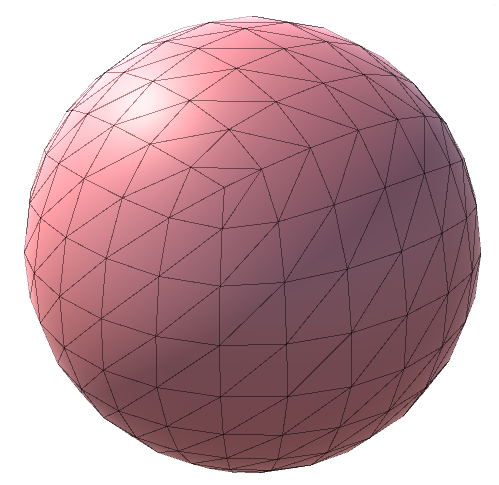
\includegraphics[height=7cm]{unity-mesh.png}
\caption{Unity sphere mesh}
\label{fig:unity-mesh}
\end{subfigure}
\hspace*{1cm}
\begin{subfigure}{7cm}
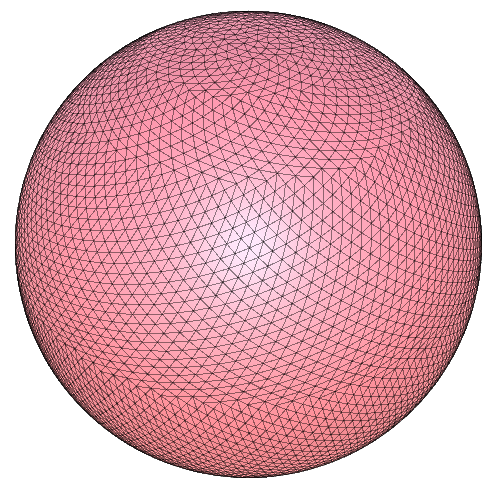
\includegraphics[height=7cm]{delaunay-mesh.png}
\caption{Delaunay mesh}
\label{fig:delaunay-mesh}
\end{subfigure}
\caption{Spherical meshes}
\label{fig:spherical-mesh}
\end{figure}
Definition and description of a 3D mesh is way beyond the scope and purpose of this document. In this context, it is simply an approximation of the sphere surface. All samples $U$ are vertices connected into triangles so that the whole sphere is covered by them without any gaps. For Driftworld, a set of prepared meshes is provided, created by \textit{Delaunay triangulation} \cite{delaunay}.

When interpolating surface data such as elevation, it is important that reasonable samples are used for the interpolation. Calculating elevation in a mountain range from a triangle with vertices too far apart may result in meaningless artifacts. Furthermore, the earlier mentioned requirement that the triangles are nearly planar would be undermined by extreme spherical triangles which exhibit considerable excess. It stands to reason that triangles used in the mesh should be as regular as possible. This is the goal and result of a Delaunay triangulation. There is a number of algorithms performing the triangulation on a plane \cite{knuth}. Since sphere has a closed mesh, an adaptation is needed.

Delaunay meshes for Driftworld use an algorithm which originally triangulates a set of random samples \cite{ma}. Because $U$ is ordered, the initial tetrahedron is somewhat difficult to construct, especially because of the requirements imposed on a spherical triangle -- in a large number of cases at least one triangle had a circumcircle larger than a great circle. For this reason, the initial structure was set to be a nearly regular octahedron with vertices assigned by a brute-force look-up. Other than that, the algorithm follows the article \cite{ma}.
\subsection{Bounding volume hiearchy}
\subsection{Collisions}

